\chapter{Introdução}
\label{chapter:introducao}
% \section{Introdução}
CubeSats são uma classe de artefatos espaciais elaborada com o intuito de reduzir custos e tempo de desenvolvimento, além de providenciar maior acessibilidade ao espaço \cite{cubesat-spec}. Inicialmente projetados para utilização educacional em universidades \cite{burt2011}, são amplamente usados para exploração espacial em órbita terrestre baixa, com altitudes entre 160km e 2000km \cite{alanazi2019}.

CubeSats possuem uma unidade básica (U) de dimensão 10cm x 10cm x 10cm e de até 1kg de massa, mas podem ser configurados em até 24 Unidades (ou 24U) \cite{cubesat}. O FloripaSat-2 \cite{floripasat2}, projeto do Laboratório de Pesquisa em Tecnologias Espaciais da UFSC no qual este trabalho se baseia, é um CubeSat 2U que se encontra no presente momento, em estágio de desenvolvimento ativo. A figura \ref{fig:floripasat2-diagram} apresenta uma renderização da configuração do FloripaSat-2.

\begin{figure}[H]
\caption{\label{fig:floripasat2-diagram}Renderização do FloripaSat-2.}
\begin{center}
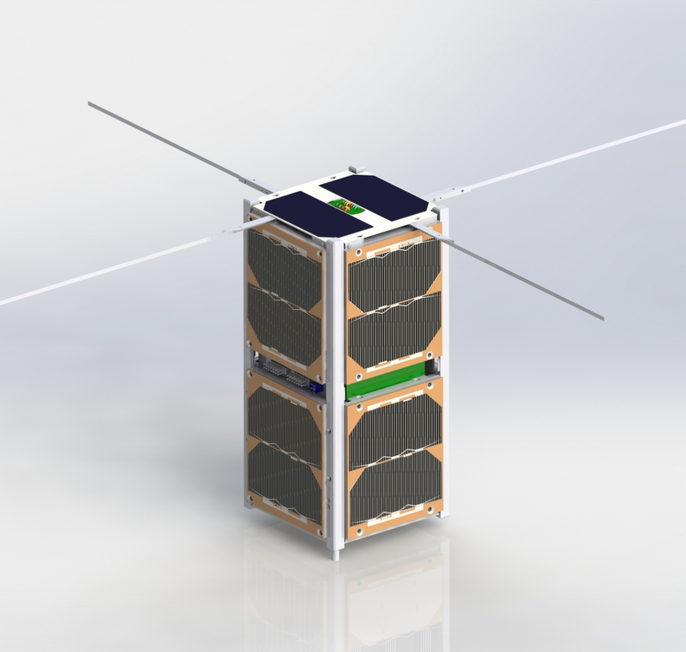
\includegraphics[scale=0.5]{images/floripasat-2-diagram.jpg}
\end{center}
\legend{Fonte: \cite{floripasat2}}
\end{figure}
\newpage

O processo de verificação de design é uma etapa crucial em projetos de engenharia.
Em tradução livre dos autores, Monteiro et al, dizem que:

\begin{citacao}
\hspace{1,2cm}Em projetos espaciais, a amplitude e cuidado minucioso dos processos de teste são ainda mais importantes, em vista do nível de confiabilidade  a ser imposto no produto final, que é comumente um artefato espacial que precisa resistir à uma gama de ameaças e funcionar em um ambientes inóspitos. \cite{aiv-cubesat}
\end{citacao}

Ainda segundo os autores, o processo de \emph{AIV} (sigla em inglês para Montagem, Integração, e Verificação) tende a ser mais leve em CubeSats, devido à menor escala dos projetos.

No entanto, o risco de um projeto de nanossatélite não é desprezível. Em um estudo realizado sobre os lançamentos de CubeSats entre 2003 e 2015, os autores \cite{panga2016} constataram que cerca de 15\% das missões CubeSat nesse período não conseguiram manter comunicações com as estações de controle, resultando em falha da missão após o lançamento.

Por esses motivos, percebe-se então a relevância de um plano de testes bem estruturado para o ciclo de desenvolvimento do FloripaSat-2. Através da elaboração e execução de testes, pretende-se elevar a confiabilidade\cite{chen-2001} do sistema, a fim de diminuir a probabilidade de que problemas no satélite resultem em falha da missão


O trabalho propõe, então, dois pontos principais:

\begin{itemize}
    \item A implementação de um sistema de workflows hospedados na plataforma GitHub Actions \cite {gh-actions} nos repositórios oficiais do projeto, que possibilite a execução automática de testes unitários nos sistemas do FloripaSat-2;
    \item A análise desritiva dos testes unitários implementados durante o desenvolvimento dos subsistemas do satélite.
\end{itemize}

Os resultados esperados deste trabalho são a criação de um modelo para automação a ser usado em futuros projetos de desenvolvimento de sistemas embarcados para CubeSats, e um relatório com as conclusões e análises obtidas por meio do estudo dos dados coletados.

\section{Objetivos}

\subsection{Objetivo Geral}

O objetivo principal do trabalho é implementar um sistema de automação dos testes unitários do firmware do FloripaSat-2 hospedado nos repositórios oficiais no \textit{GitHub}. Esses \textit{workflows} serão empregados durante o ciclo de desenvolvimento da missão, executando os testes de forma automática seguindo os critérios de execução estabelecidos pelo projeto.

\subsection{Objetivos Específicos}

\begin{enumerate}
    \item Apresentar uma introdução ao estado da arte referente a testes de software, desenvolvimento de CubeSats e relacionar os dois temas no contexto do FloripaSat-2;
    \item Implementar \textit{workflows} capazes de automatizar a execução de testes unitários;
    \item Apresentar um estudo sobre os testes dos sistemas do FloripaSat-2 que foram implementados durante o andamento do projeto;
    \item Disponibilizar códigos-fonte, dados de registro e resultados obtidos.
\end{enumerate}
\section{Organização do trabalho}

Este trabalho está organizado do seguinte modo:

\begin{itemize}
    \item O capítulo \ref{chapter:fundamentacao} apresenta a definição da metodologia utilizada e a formalização da fundamentação teórica utilizada na elaboração do trabalho;
    \item O capítulo \ref{chapter:relacionados} apresenta uma breve revisão de alguns trabalhos relacionados que abordam o desenvolvimento e testes de CubeSats;
    \item O capítulo \ref{chapter:proposta} apresenta e descreve o sistema proposto;
    \item O capítulo \ref{chapter:projeto} apresenta a descrição formal da implementação do sistema
    \item O capítulo \ref{chapter:resultados} apresenta uma análise dos resultados observados
    \item O capítulo \ref{chapter:conclusao} traz as conclusões e considerações sobre o trabalho, e explora possíveis trabalhos futuros
\end{itemize}
